\documentclass[11pt,twoside]{clrdsbook}
% \documentclass[tikz,border=40mm]{standalone}
% \usetikzlibrary{shapes,calc}
% \usepackage{anyfontsize}
%\usepackage{mathptmx}
%\begin{document}
\newcommand{\ElemLabel}[4]{
    \begin{minipage}{2.2cm}
        \centering
        {{\fontsize{13}{13}\selectfont\bfseries #1} \hfill {\fontsize{12}{12}\selectfont #2}}\\[1ex]
        {\fontsize{36}{36}\selectfont \bfseries #3}\\[2ex]
        {\fontsize{13}{13}\selectfont  \sffamily #4}
    \end{minipage}
}

\newcommand{\NaturalElem}[4]{\ElemLabel{#1}{#2}{#3}{#4}}

\newcommand{\SyntheticElem}[4]{\ElemLabel{#1}{#2}{\color{gray}#3}{\color{gray}#4}}

\newcommand{\TablaPeriodica}[1][0.55]{
    \begin{tikzpicture}[font=\normalfont,scale=#1, transform shape]

        % Fill Color Styles
        \tikzstyle{ElementFill} = [fill=gray!40]
        \tikzstyle{AlkaliMetalFill} = [fill=RoyalPurple!40]
        \tikzstyle{AlkalineEarthMetalFill} = [fill=RoyalBlue!40]
        \tikzstyle{MetalFill} = [fill=SkyBlue!40]
        \tikzstyle{MetalloidFill} = [fill=LimeGreen!55]
        \tikzstyle{NonmetalFill} = [fill=Orange!55]
        \tikzstyle{HalogenFill} = [fill=BrickRed!55]
        \tikzstyle{NobleGasFill} = [fill=Goldenrod!40]
        \tikzstyle{LanthanideActinideFill} = [fill=teal!40]

        % Element Styles
        \tikzstyle{Element} = [ElementFill,
        minimum width=2.5cm, minimum height=2.5cm, node distance=2.75cm]
        \tikzstyle{AlkaliMetal} = [Element, AlkaliMetalFill]
        \tikzstyle{AlkalineEarthMetal} = [Element, AlkalineEarthMetalFill]
        \tikzstyle{Metal} = [Element, MetalFill]
        \tikzstyle{Metalloid} = [Element, MetalloidFill]
        \tikzstyle{Nonmetal} = [Element, NonmetalFill]
        \tikzstyle{Halogen} = [Element, HalogenFill]
        \tikzstyle{NobleGas} = [Element, NobleGasFill]
        \tikzstyle{LanthanideActinide} = [Element, LanthanideActinideFill]
        \tikzstyle{PeriodLabel} = [font={\sffamily\LARGE}, node distance=2.0cm]
        \tikzstyle{GroupLabel} = [font={\sffamily\LARGE}, minimum width=2.75cm, node distance=2.0cm]

        % Group 1 - IA
        \node[Element] (H) {\NaturalElem{1} {1.0079}{H}{Hidr\'ogeno}};
        \node[below of=H, AlkaliMetal] (Li) {\NaturalElem{3}{6.941}{Li}{Litio}};
        \node[below of=Li, AlkaliMetal] (Na) {\NaturalElem{11}{22.990}{Na}{Sodio}};
        \node[below of=Na, AlkaliMetal] (K) {\NaturalElem{19}{39.098}{K}{Potasio}};
        \node[below of=K, AlkaliMetal] (Rb) {\NaturalElem{37}{85.468}{Rb}{Rubidio}};
        \node[below of=Rb, AlkaliMetal] (Cs) {\NaturalElem{55}{132.91}{Cs}{Cesio}};
        \node[below of=Cs, AlkaliMetal] (Fr) {\NaturalElem{87}{223}{Fr}{Francio}};

        % Group 2 - IIA
        \node[right of=Li, AlkalineEarthMetal] (Be) {\NaturalElem{4}{9.0122}{Be}{Berilio}};
        \node[below of=Be, AlkalineEarthMetal] (Mg) {\NaturalElem{12}{24.305}{Mg}{Magnesio}};
        \node[below of=Mg, AlkalineEarthMetal] (Ca) {\NaturalElem{20}{40.078}{Ca}{Calcio}};
        \node[below of=Ca, AlkalineEarthMetal] (Sr) {\NaturalElem{38}{87.62}{Sr}{Stroncio}};
        \node[below of=Sr, AlkalineEarthMetal] (Ba) {\NaturalElem{56}{137.33}{Ba}{Bario}};
        \node[below of=Ba, AlkalineEarthMetal] (Ra) {\NaturalElem{88}{226}{Ra}{Radio}};

        % Group 3 - IIIB
        \node[right of=Ca, Metal] (Sc) {\NaturalElem{21}{44.956}{Sc}{Escandio}};
        \node[below of=Sc, Metal] (Y) {\NaturalElem{39}{88.906}{Y}{Itrio}};
        \node[below of=Y, LanthanideActinide] (LaLu) {\NaturalElem{57-71}{}{*}{Lant\'anido}};
        \node[below of=LaLu, LanthanideActinide] (AcLr) {\NaturalElem{89-103}{}{**}{Act\'inido}};

        % Group 4 - IVB
        \node[right of=Sc, Metal] (Ti) {\NaturalElem{22}{47.867}{Ti}{Titanio}};
        \node[below of=Ti, Metal] (Zr) {\NaturalElem{40}{91.224}{Zr}{Circonio}};
        \node[below of=Zr, Metal] (Hf) {\NaturalElem{72}{178.49}{Hf}{Hafnio}};
        \node[below of=Hf, Metal] (Rf) {\SyntheticElem{104}{261}{Rf}{Rutherfordio}};

        % Group 5 - VB
        \node[right of=Ti, Metal] (V) {\NaturalElem{23}{50.942}{V}{Vanadio}};
        \node[below of=V, Metal] (Nb) {\NaturalElem{41}{92.906}{Nb}{Niobio}};
        \node[below of=Nb, Metal] (Ta) {\NaturalElem{73}{180.95}{Ta}{Tantalo}};
        \node[below of=Ta, Metal] (Db) {\SyntheticElem{105}{262}{Db}{Dubnio}};

        % Group 6 - VIB
        \node[right of=V, Metal] (Cr) {\NaturalElem{24}{51.996}{Cr}{Cromo}};
        \node[below of=Cr, Metal] (Mo) {\NaturalElem{42}{95.94}{Mo}{Molybdeno}};
        \node[below of=Mo, Metal] (W) {\NaturalElem{74}{183.84}{W}{Tungstenio}};
        \node[below of=W, Metal] (Sg) {\SyntheticElem{106}{266}{Sg}{Seaborgio}};

        % Group 7 - VIIB
        \node[right of=Cr, Metal] (Mn) {\NaturalElem{25}{54.938}{Mn}{Manganeso}};
        \node[below of=Mn, Metal] (Tc) {\NaturalElem{43}{96}{Tc}{Tecnecio}};
        \node[below of=Tc, Metal] (Re) {\NaturalElem{75}{186.21}{Re}{Renio}};
        \node[below of=Re, Metal] (Bh) {\SyntheticElem{107}{264}{Bh}{Bohrio}};

        % Group 8 - VIIIB
        \node[right of=Mn, Metal] (Fe) {\NaturalElem{26}{55.845}{Fe}{Hierro}};
        \node[below of=Fe, Metal] (Ru) {\NaturalElem{44}{101.07}{Ru}{Ruthenio}};
        \node[below of=Ru, Metal] (Os) {\NaturalElem{76}{190.23}{Os}{Osmio}};
        \node[below of=Os, Metal] (Hs) {\SyntheticElem{108}{277}{Hs}{Hassio}};

        % Group 9 - VIIIB
        \node[right of=Fe, Metal] (Co) {\NaturalElem{27}{58.933}{Co}{Cobalto}};
        \node[below of=Co, Metal] (Rh) {\NaturalElem{45}{102.91}{Rh}{Rodio}};
        \node[below of=Rh, Metal] (Ir) {\NaturalElem{77}{192.22}{Ir}{Iridio}};
        \node[below of=Ir, Metal] (Mt) {\SyntheticElem{109}{268}{Mt}{Meitnerio}};

        % Group 10 - VIIIB
        \node[right of=Co, Metal] (Ni) {\NaturalElem{28}{58.693}{Ni}{Niquel}};
        \node[below of=Ni, Metal] (Pd) {\NaturalElem{46}{106.42}{Pd}{Paladio}};
        \node[below of=Pd, Metal] (Pt) {\NaturalElem{78}{195.08}{Pt}{Platino}};
        \node[below of=Pt, Metal] (Ds) {\SyntheticElem{110}{281}{Ds}{Darmstadtio}};

        % Group 11 - IB
        \node[right of=Ni, Metal] (Cu) {\NaturalElem{29}{63.546}{Cu}{Cobre}};
        \node[below of=Cu, Metal] (Ag) {\NaturalElem{47}{107.87}{Ag}{Plata}};
        \node[below of=Ag, Metal] (Au) {\NaturalElem{79}{196.97}{Au}{Oro}};
        \node[below of=Au, Metal] (Rg) {\SyntheticElem{111}{280}{Rg}{Roentgenio}};

        % Group 12 - IIB
        \node[right of=Cu, Metal] (Zn) {\NaturalElem{30}{65.39}{Zn}{Zinc}};
        \node[below of=Zn, Metal] (Cd) {\NaturalElem{48}{112.41}{Cd}{Cadmio}};
        \node[below of=Cd, Metal] (Hg) {\NaturalElem{80}{200.59}{Hg}{Mercurio}};
        \node[below of=Hg, Metal] (Cn) {\SyntheticElem{112}{285}{Cn}{Copernicio}};

        % Group 13 - IIIA
        \node[right of=Zn, Metal] (Ga) {\NaturalElem{31}{69.723}{Ga}{Galio}};
        \node[above of=Ga, Metal] (Al) {\NaturalElem{13}{26.982}{Al}{Aluminio}};
        \node[above of=Al, Metalloid] (B) {\NaturalElem{5}{10.811}{B}{Boro}};
        \node[below of=Ga, Metal] (In) {\NaturalElem{49}{114.82}{In}{Indo}};
        \node[below of=In, Metal] (Tl) {\NaturalElem{81}{204.38}{Tl}{Talio}};
        \node[below of=Tl, Metal] (Nh) {\SyntheticElem{113}{284}{Nh}{Nihonio}};

        % Group 14 - IVA
        \node[right of=B, Nonmetal] (C) {\NaturalElem{6}{12.011}{C}{Carbono}};
        \node[below of=C, Metalloid] (Si) {\NaturalElem{14}{28.086}{Si}{Silicio}};
        \node[below of=Si, Metalloid] (Ge) {\NaturalElem{32}{72.64}{Ge}{Germanio}};
        \node[below of=Ge, Metal] (Sn) {\NaturalElem{50}{118.71}{Sn}{Esta\~no}};
        \node[below of=Sn, Metal] (Pb) {\NaturalElem{82}{207.2}{Pb}{Plomo}};
        \node[below of=Pb, Metal] (Fl) {\SyntheticElem{114}{289}{Fl}{Flerovio}};

        % Group 15 - VA
        \node[right of=C, Nonmetal] (N) {\NaturalElem{7}{14.007}{N}{Nitr\'ogeno}};
        \node[below of=N, Nonmetal] (P) {\NaturalElem{15}{30.974}{P}{F\'osforo}};
        \node[below of=P, Metalloid] (As) {\NaturalElem{33}{74.922}{As}{Ars\'enico}};
        \node[below of=As, Metalloid] (Sb) {\NaturalElem{51}{121.76}{Sb}{Antimonio}};
        \node[below of=Sb, Metal] (Bi) {\NaturalElem{83}{208.98}{Bi}{Bismuto}};
        \node[below of=Bi, Metal] (Mc) {\SyntheticElem{115}{288}{Mc}{Moscovio}};

        % Group 16 - VIA
        \node[right of=N, Nonmetal] (O) {\NaturalElem{8}{15.999}{O}{Ox\'igeno}};
        \node[below of=O, Nonmetal] (S) {\NaturalElem{16}{32.065}{S}{Az\'ufre}};
        \node[below of=S, Nonmetal] (Se) {\NaturalElem{34}{78.96}{Se}{Selenio}};
        \node[below of=Se, Metalloid] (Te) {\NaturalElem{52}{127.6}{Te}{Tellurio}};
        \node[below of=Te, Metalloid] (Po) {\NaturalElem{84}{209}{Po}{Polonio}};
        \node[below of=Po, Metal] (Lv) {\SyntheticElem{116}{293}{Lv}{Libermonio}};

        % Group 17 - VIIA
        \node[right of=O, Halogen] (F) {\NaturalElem{9}{18.998}{F}{Fluor}};
        \node[below of=F, Halogen] (Cl) {\NaturalElem{17}{35.453}{Cl}{Cloro}};
        \node[below of=Cl, Halogen] (Br) {\NaturalElem{35}{79.904}{Br}{Bromo}};
        \node[below of=Br, Halogen] (I) {\NaturalElem{53}{126.9}{I}{Yodo}};
        \node[below of=I, Halogen] (At) {\NaturalElem{85}{210}{At}{\'Astato}};
        \node[below of=At, Element] (Ts) {\SyntheticElem{117}{292}{Ts}{Teneso}};

        % Group 18 - VIIIA
        \node[right of=F, NobleGas] (Ne) {\NaturalElem{10}{20.180}{Ne}{Ne\'on}};
        \node[above of=Ne, NobleGas] (He) {\NaturalElem{2}{4.0025}{He}{Helio}};
        \node[below of=Ne, NobleGas] (Ar) {\NaturalElem{18}{39.948}{Ar}{Arg\'on}};
        \node[below of=Ar, NobleGas] (Kr) {\NaturalElem{36}{83.8}{Kr}{Kript\'on}};
        \node[below of=Kr, NobleGas] (Xe) {\NaturalElem{54}{131.29}{Xe}{Xen\'on}};
        \node[below of=Xe, NobleGas] (Rn) {\NaturalElem{86}{222}{Rn}{Rad\'on}};
        \node[below of=Rn, Nonmetal] (Og) {\SyntheticElem{118}{294}{Og}{Oganesón}};

        % Period
        \node[left of=H, PeriodLabel] (Period1) {1};
        \node[left of=Li, PeriodLabel] (Period2) {2};
        \node[left of=Na, PeriodLabel] (Period3) {3};
        \node[left of=K, PeriodLabel] (Period4) {4};
        \node[left of=Rb, PeriodLabel] (Period5) {5};
        \node[left of=Cs, PeriodLabel] (Period6) {6};
        \node[left of=Fr, PeriodLabel] (Period7) {7};

        % Group
        \node[above of=H, GroupLabel] (Group1) {1 \hfill IA};
        \node[above of=Be, GroupLabel] (Group2) {2 \hfill IIA};
        \node[above of=Sc, GroupLabel] (Group3) {3 \hfill IIIA};
        \node[above of=Ti, GroupLabel] (Group4) {4 \hfill IVB};
        \node[above of=V, GroupLabel] (Group5) {5 \hfill VB};
        \node[above of=Cr, GroupLabel] (Group6) {6 \hfill VIB};
        \node[above of=Mn, GroupLabel] (Group7) {7 \hfill VIIB};
        \node[above of=Fe, GroupLabel] (Group8) {8 \hfill VIIIB};
        \node[above of=Co, GroupLabel] (Group9) {9 \hfill VIIIB};
        \node[above of=Ni, GroupLabel] (Group10) {10 \hfill VIIIB};
        \node[above of=Cu, GroupLabel] (Group11) {11 \hfill IB};
        \node[above of=Zn, GroupLabel] (Group12) {12 \hfill IIB};
        \node[above of=B, GroupLabel] (Group13) {13 \hfill IIIA};
        \node[above of=C, GroupLabel] (Group14) {14 \hfill IVA};
        \node[above of=N, GroupLabel] (Group15) {15 \hfill VA};
        \node[above of=O, GroupLabel] (Group16) {16 \hfill VIA};
        \node[above of=F, GroupLabel] (Group17) {17 \hfill VIIA};
        \node[above of=He, GroupLabel] (Group18) {18 \hfill VIIIA};


        % Lanthanide
        \node[below of=Rf, LanthanideActinide, yshift=-1cm] (La) {\NaturalElem{57}{138.91}{La}{Lant\'anido}};
        \node[right of=La, LanthanideActinide] (Ce) {\NaturalElem{58}{140.12}{Ce}{Cerio}};
        \node[right of=Ce, LanthanideActinide] (Pr) {\NaturalElem{59}{140.91}{Pr}{Praseodymio}};
        \node[right of=Pr, LanthanideActinide] (Nd) {\NaturalElem{60}{144.24}{Nd}{Neodimio}};
        \node[right of=Nd, LanthanideActinide] (Pm) {\NaturalElem{61}{145}{Pm}{Prometio}};
        \node[right of=Pm, LanthanideActinide] (Sm) {\NaturalElem{62}{150.36}{Sm}{Samario}};
        \node[right of=Sm, LanthanideActinide] (Eu) {\NaturalElem{63}{151.96}{Eu}{Europio}};
        \node[right of=Eu, LanthanideActinide] (Gd) {\NaturalElem{64}{157.25}{Gd}{Gadolinio}};
        \node[right of=Gd, LanthanideActinide] (Tb) {\NaturalElem{65}{158.93}{Tb}{Terbio}};
        \node[right of=Tb, LanthanideActinide] (Dy) {\NaturalElem{66}{162.50}{Dy}{Disprosio}};
        \node[right of=Dy, LanthanideActinide] (Ho) {\NaturalElem{67}{164.93}{Ho}{Holmio}};
        \node[right of=Ho, LanthanideActinide] (Er) {\NaturalElem{68}{167.26}{Er}{Erbio}};
        \node[right of=Er, LanthanideActinide] (Tm) {\NaturalElem{69}{168.93}{Tm}{Tulio}};
        \node[right of=Tm, LanthanideActinide] (Yb) {\NaturalElem{70}{173.04}{Yb}{Yterbio}};
        \node[right of=Yb, LanthanideActinide] (Lu) {\NaturalElem{71}{174.97}{Lu}{Luterio}};

        % Actinide
        \node[below of=La, LanthanideActinide] (Ac) {\NaturalElem{89}{227}{Ac}{Actinio}};
        \node[right of=Ac, LanthanideActinide]              (Th) {\NaturalElem{90}{232.04}{Th}{Torio}};
        \node[right of=Th, LanthanideActinide]              (Pa) {\NaturalElem{91}{231.04}{Pa}{Protactinio}};
        \node[right of=Pa, LanthanideActinide]              (U)  {\NaturalElem{92}{238.03}{U}{Uranio}};
        \node[right of=U, LanthanideActinide]               (Np) {\SyntheticElem{93}{237}{Np}{Neptunio}};
        \node[right of=Np, LanthanideActinide]              (Pu) {\SyntheticElem{94}{244}{Pu}{Plutonio}};
        \node[right of=Pu, LanthanideActinide]              (Am) {\SyntheticElem{95}{243}{Am}{Americio}};
        \node[right of=Am, LanthanideActinide]              (Cm) {\SyntheticElem{96}{247}{Cm}{Curio}};
        \node[right of=Cm, LanthanideActinide]              (Bk) {\SyntheticElem{97}{247}{Bk}{Berkelio}};
        \node[right of=Bk, LanthanideActinide]              (Cf) {\SyntheticElem{98}{251}{Cf}{Californio}};
        \node[right of=Cf, LanthanideActinide]              (Es) {\SyntheticElem{99}{252}{Es}{Einsteinio}};
        \node[right of=Es, LanthanideActinide]              (Fm) {\SyntheticElem{100}{257}{Fm}{Fermio}};
        \node[right of=Fm, LanthanideActinide]              (Md) {\SyntheticElem{101}{258}{Md}{Mendelevio}};
        \node[right of=Md, LanthanideActinide]              (No) {\SyntheticElem{102}{259}{No}{Nobelio}};
        \node[right of=No, LanthanideActinide]              (Lr) {\SyntheticElem{103}{262}{Lr}{Lawrencio}};

        % Draw dotted lines connecting Lanthanide breakout to main table
        \draw[thick,dotted] (LaLu.north east) -- (La.north west)
        (LaLu.south west) -- (La.south west);
        % Draw dotted lines connecting Actinide breakout to main table
        \draw[thick,dotted] (AcLr.north east) -- (Ac.north west)
        (AcLr.south west) -- (Ac.south west);

        % Legend
        \fill[AlkaliMetalFill] ($(La -| Period7.west) + (0em,2em)$)
        rectangle +(2em, 2em) node[right, yshift=-2ex]  (AlkaliMetal) {\fontsize{20}{20}\selectfont \bfseries Metales Alcalinos};
        \fill[AlkalineEarthMetalFill] ($(AlkaliMetal.west) - (2em,4em)$)
        rectangle +(2em, 2em) node[right, yshift=-2ex] (AlkalineEarthMetal) {\fontsize{20}{20}\selectfont \bfseries Metales Alcalino-terreos};
        \fill[MetalFill] ($(AlkalineEarthMetal.west) - (2em,4em)$)
        rectangle +(2em, 2em) node[right, yshift=-2ex] (Metal) {\fontsize{20}{20}\selectfont \bfseries Metal};
        \fill[MetalloidFill] ($(Metal.west) - (2em,4em)$)
        rectangle +(2em, 2em) node[right, yshift=-2ex] (Metalloid) {\fontsize{20}{20}\selectfont \bfseries Metaloide};
        \fill[NonmetalFill] ($(Metalloid.west) - (2em,4em)$)
        rectangle +(2em, 2em) node[right, yshift=-2ex] (Non-metal) {\fontsize{20}{20}\selectfont \bfseries No metal};
        \fill[HalogenFill] ($(Non-metal.west) - (2em,4em)$)
        rectangle +(2em, 2em) node[right, yshift=-2ex] (Halogen) {\fontsize{20}{20}\selectfont \bfseries Hal\'ogeno};
        \fill[NobleGasFill] ($(Halogen.west) - (2em,4em)$)
        rectangle +(2em, 2em) node[right, yshift=-2ex] (NobleGas) {\fontsize{20}{20}\selectfont \bfseries Gases Nobles};
        \fill[LanthanideActinideFill] ($(NobleGas.west) - (2em,4em)$)
        rectangle +(2em, 2em) node[right, yshift=-2ex] (Lanthanide/Actinide) {\fontsize{20}{20}\selectfont \bfseries Lant\'anidos/Act\'inidos};

        \node at (Li -| V) [draw, Element, fill=white] (legend) {\NaturalElem{Z}{$A_r$}{\fontsize{36}{36}\selectfont S}{Símbolo}};
        \node[align=left,xshift=2mm] at (Li -| Cr.east) {\fontsize{20}{20}\selectfont \bfseries Negro: Naturales \\ {\fontsize{20}{20}\selectfont \bfseries\color{gray}Gris: Sint\'eticos}};
        \node[align=center] at (H -| Cr) {\fontsize{36}{6}\selectfont  \bfseries Simbología:};

        % Diagram Title
        % \node at (H.west -| Fe.north) [scale=2, font={\sffamily\Huge\bfseries}]
        % {Tabla Peri\'odica de los Elementos};

    \end{tikzpicture}
}
%\end{document}
\title{Cuaderno de Trabajo}
\subject{Química 3}
\grade{3$^\circ$ de Secundaria}
\author{J. C. Melchor Pinto}

\begin{document}
\dominitoc[n]%% Crea minitoc
\maketitle%% Crea la portada
\tableofcontents%% Crea el índice
\thispagestyle{empty} \mbox{}
\newpage

\mychapter{}

\thispagestyle{plain}
\section{Los materiales, las sustancias y sus propiedades}
This is a sample of a section
\subsection{¿Cómo sabemos que un material es distinto de otro?}
\subsection{¿Cómo podemos medir las propiedades de los materiales?}
\newpage

\thispagestyle{plain}
\section{Recta Num\'erica, Densidad y Orden}

La recta numérica es una línea recta en la que se representan los números reales. La recta numérica es una forma de representar los números reales en una línea recta. En ella, cada punto representa un número real. Los números se pueden representar y se pueden comparar los números reales en la recta numérica.
Para poder trabajar con números enteros de manera efectiva, es fundamental ordenarlos en la recta numérica. Los números positivos se ubican hacia la derecha, mientras que los números negativos se colocan hacia la izquierda. Veamos algunos ejemplos:

\subsection{Orden de los números enteros}
\subsubsection{Orden de los números enteros positivos}
Ordenemos los siguientes números positivos: $3, 7, 1, 5$.

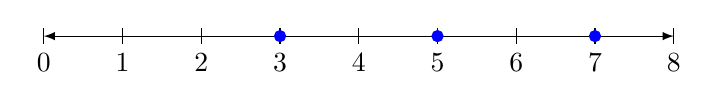
\begin{tikzpicture}
    % Numeric line
    \draw[latex-latex] (0,0) -- (8,0);
    \foreach \x in {0,1,2,3,4,5,6,7,8}
    \draw (\x,0.1) -- (\x,-0.1);
    \foreach \x/\label in {0/0,1/1,2/2,3/3,4/4,5/5,6/6,7/7,8/8}
    \node[below] at (\x,-0.1) {$\label$};

    % Marking positive numbers
    \foreach \x in {3,5,7}
    \filldraw[blue] (\x,0) circle (2pt);
\end{tikzpicture}

Los números positivos ordenados son: $1, 3, 5, 7$.

\subsubsection{Orden de los números enteros negativos}

Ahora, ordenemos los siguientes números negativos: $-4, -1, -3, -2$.
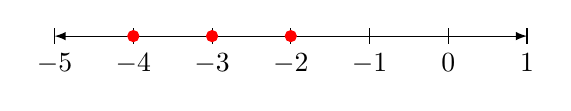
\begin{tikzpicture}
    % Numeric line
    \draw[latex-latex] (-5,0) -- (1,0);
    \foreach \x in {-5,-4,-3,-2,-1,0,1}
    \draw (\x,0.1) -- (\x,-0.1);
    \foreach \x/\label in {-5/-5,-4/-4,-3/-3,-2/-2,-1/-1,0/0,1/1}
    \node[below] at (\x,-0.1) {$\label$};

    % Marking negative numbers
    \foreach \x in {-4,-3,-2}
    \filldraw[red] (\x,0) circle (2pt);
\end{tikzpicture}

Los números negativos ordenados son: $-4, -3, -2, -1$.

\subsection{Orden de fracciones y decimales}

\subsubsection{Orden en los n\'umeros fraccionarios}
Para comparar fracciones, debemos convertirlas a un mismo denominador. Por ejemplo, para comparar $\frac{1}{2}$ y $\frac{3}{4}$, debemos convertirlas a un mismo denominador. El mínimo común múltiplo de $2$ y $4$ es $4$, por lo que debemos convertir $\frac{1}{2}$ a $\frac{2}{4}$, y $\frac{3}{4}$ a $\frac{3}{4}$. Ahora podemos compararlas, y vemos que:

\[\frac{2}{4}<\frac{3}{4}\]

\begin{center}
    \begin{tikzpicture}[scale=1]
        % Recta numérica
        \draw[latex-latex] (-0.8,0) -- (10.2,0);

        % Números racionales entre 0 y 1
        \foreach \x in {0,2.5,5,7.5,10}
        \draw (\x,0.1) -- (\x,-0.1);

        % Etiquetas de números racionales
        \foreach \x/\label in { 0/{0}, 2.5/{\dfrac{1}{4}}, 5/{{\color{gray}\dfrac{1}{2}=}\dfrac{2}{4}}, 7.5/{\dfrac{3}{4}},10/{1}}
        \node[below] at (\x,-0.1) {$\label$};

        % Puntos rojo y verde
        \fill[color=red!50!black] (5,0) circle (0.16);
        \fill[color=red!50!black] (7.5,0) circle (0.16);
    \end{tikzpicture}
\end{center}

\subsubsection{Orden en los n\'umeros decimales}

Para comparar decimales, debemos convertirlos a un mismo número de decimales. Por ejemplo, para comparar $0.5$ y $0.35$, debemos convertirlos a un mismo número de decimales. El número de decimales de $0.5$ es $1$, y el número de decimales de $0.35$ es $2$. Para convertir $0.5$ a $0.50$, debemos agregar un $0$ al final. Ahora podemos compararlos, y vemos que:

\[0.50>0.35\]

\begin{center}
    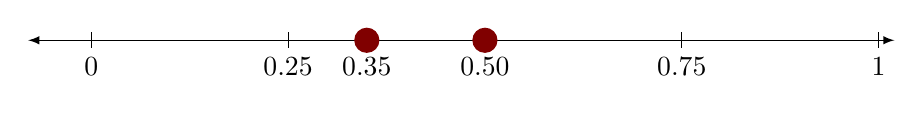
\begin{tikzpicture}[scale=1]
        % Recta numérica
        \draw[latex-latex] (-0.8,0) -- (10.2,0);

        % Números racionales entre 0 y 1
        \foreach \x in {0,2.5,5,7.5,10}
        \draw (\x,0.1) -- (\x,-0.1);

        % Etiquetas de números racionales
        \foreach \x/\label in { 0/{0}, 2.5/{0.25}, 3.5/{0.35}, 5/{0.50}, 7.5/{0.75},10/{1}}
        \node[below] at (\x,-0.1) {$\label$};

        % Puntos rojo y verde
        \fill[color=red!50!black] (5,0) circle (0.16);
        \fill[color=red!50!black] (3.5,0) circle (0.16);
    \end{tikzpicture}
\end{center}

\subsection{Densidad de fracciones y decimales}

En teoría de conjuntos, se dice que un conjunto numérico es \textbf{denso}, si entre dos elementos cualesquiera del conjunto, existe otro elemento del conjunto. Por ejemplo, el conjunto de los números racionales es denso, porque entre dos números racionales cualesquiera, existe otro número racional.

Por ejemplo, entre $\frac{1}{2}$ y $\frac{3}{4}$, existe $\frac{5}{8}$.\\

% Representacion detallada en Tikz de una recta numérica que muestra la densidad de los números racionales. 
% Se muestra la recta numérica con los números racionales entre 0 y 1, y se muestra con etiquetas que entre dos números racionales como el 1/2 y  el 3/4,
% existe otro número racional como el 5/8.
\begin{tikzpicture}[scale=2]
    % Recta numérica
    \draw[latex-latex] (4,0) -- (8,0);

    % Números racionales entre 0 y 1
    \foreach \x in { 5, 6, 7  }
    \draw (\x,0.1) -- (\x,-0.1);

    % Etiquetas de números racionales
    \foreach \x/\label in { 5/{\dfrac{1}{2}}, 6.25/{\dfrac{5}{8}}, 7.5/{\dfrac{3}{4}}}
    \node[below] at (\x,-0.1) {$\label$};

    % Puntos rojo y verde
    \fill[color=red!50!black] (5,0) circle (0.08);
    \fill[color=red!50!black] (7.5,0) circle (0.08);
    \fill[color=green!50!black] (6.25,0) circle (0.08);
\end{tikzpicture}

Si observamos ahora en medio del $\frac{1}{2}$ y el $\frac{5}{8}$, está el $\frac{9}{16}$.\\

% Representacion detallada en Tikz de una recta numérica que muestra la densidad de los números racionales. 
% Se muestra la recta numérica con los números racionales entre 0 y 1, y se muestra con etiquetas que entre dos números racionales como el 1/2 y  el 5/8,
% existe otro número racional como el 9/16
\begin{tikzpicture}[scale=2]
    % Recta numérica
    \draw[latex-latex] (4,0) -- (8,0);

    % Números racionales entre 0 y 1
    \foreach \x in {  5, 6, 7}
    \draw (\x,0.1) -- (\x,-0.1);

    % Etiquetas de números racionales
    \foreach \x/\label in {5/{\dfrac{1}{2}}, 5.625/{\dfrac{9}{16}}, 6.25/{\dfrac{5}{8}}, 7.5/{\dfrac{3}{4}}}
    \node[below] at (\x,-0.1) {$\label$};

    % Puntos rojo y verde
    \fill[color=red!50!black] (5,0) circle (0.08);
    \fill[color=green!50!black] (6.25,0) circle (0.08);
    \fill[color=red!50!black] (7.5,0) circle (0.08);
    \fill[color=blue!50!black] (5.625,0) circle (0.08);
\end{tikzpicture}

Y si observamos ahora en medio del $\frac{1}{2}$ y el $\frac{9}{16}$, esta el $\frac{19}{32}$.\\

% Representacion detallada en Tikz de una recta numérica que muestra la densidad de los números racionales.
% Se muestra la recta numérica con los números racionales entre 0 y 1, y se muestra con etiquetas que entre dos números racionales como el 1/2 y  el 9/16,
% existe otro número racional como el 19/32

\begin{tikzpicture}[scale=2]
    % Recta numérica
    \draw[latex-latex] (4,0) -- (8,0);

    % Números racionales entre 0 y 1
    \foreach \x in {  5, 6, 7}
    \draw (\x,0.1) -- (\x,-0.1);

    % Etiquetas de números racionales
    \foreach \x/\label in {5/{\dfrac{1}{2}}, 5.3125/{\dfrac{19}{32}}, 5.625/{\dfrac{9}{16}}, 6.25/{\dfrac{5}{8}}, 7.5/{\dfrac{3}{4}}}
    \node[below] at (\x,-0.1) {$\label$};
    % Puntos rojo y verde
    \fill[color=red!50!black] (5,0) circle (0.08);
    \fill[color=green!50!black] (6.25,0) circle (0.08);
    \fill[color=red!50!black] (7.5,0) circle (0.08);
    \fill[color=blue!50!black] (5.625,0) circle (0.08);
    \fill[color=yellow!50!black] (5.3125,0) circle (0.08);
\end{tikzpicture}

\subsubsection{Densidad de los decimales}
Los decimales también son densos. Por ejemplo, entre $0.5$ y $0.6$, existe $0.55$.\\

% Representacion detallada en Tikz de una recta numérica que muestra la densidad de los números decimales.
% Se muestra la recta numérica con los números decimales entre 0 y 1, y se muestra con etiquetas que entre dos números decimales como el 0.5 y  el 0.6,
% existe otro número decimal como el 0.55
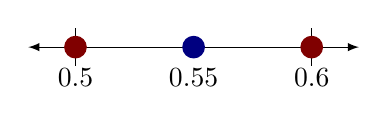
\begin{tikzpicture}[scale=3]
    % Recta numérica
    \draw[latex-latex] (4.8,0) -- (6.2,0);

    % Números decimales entre 0 y 1
    \foreach \x in {  5, 6}
    \draw (\x,0.08) -- (\x,-0.08);

    % Etiquetas de números decimales
    \foreach \x/\label in {5/{0.5}, 5.5/{0.55}, 6/{0.6}}
    \node[below] at (\x,-0.05) {$\label$};

    % Puntos rojo y verde
    \fill[color=red!50!black] (5,0) circle (0.048);
    \fill[color=red!50!black] (6,0) circle (0.048);
    \fill[color=blue!50!black] (5.5,0) circle (0.048);
\end{tikzpicture}

Si observamos de cerca ahora en medio del $0.5$ y el $0.55$, esta el $0.525$.\\

% Representacion detallada en Tikz de una recta numérica que muestra la densidad de los números decimales.
% Se muestra la recta numérica con los números decimales entre 0 y 1, y se muestra con etiquetas que entre dos números decimales como el 0.5 y  el 0.55,
% existe otro número decimal como el 0.525
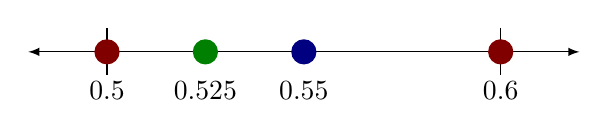
\begin{tikzpicture}[scale=5]
    % Recta numérica
    \draw[latex-latex] (4.8,0) -- (6.2,0);
    % Números decimales entre 0 y 1
    \foreach \x in {  5, 6}
    \draw (\x,0.06) -- (\x,-0.06);
    % Etiquetas de números decimales
    \foreach \x/\label in {5/{0.5}, 5.25/{0.525}, 5.5/{0.55}, 6/{0.6}}
    \node[below] at (\x,-0.05) {$\label$};
    % Puntos rojo y verde
    \fill[color=red!50!black] (5,0) circle (0.032);
    \fill[color=red!50!black] (6,0) circle (0.032);
    \fill[color=blue!50!black] (5.5,0) circle (0.032);
    \fill[color=green!50!black] (5.25,0) circle (0.032);
\end{tikzpicture}

Y si observamos de cerca ahora en medio del $0.5$ y el $0.525$, esta el $0.5125$.\\

% Representacion detallada en Tikz de una recta numérica que muestra la densidad de los números decimales.
% Se muestra la recta numérica con los números decimales entre 0 y 1, y se muestra con etiquetas que entre dos números decimales como el 0.5 y  el 0.525,
% existe otro número decimal como el 0.5125
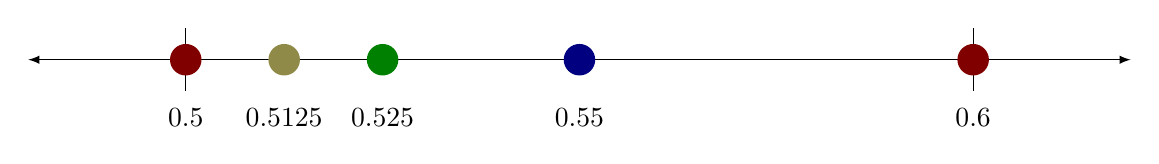
\begin{tikzpicture}[scale=10]
    % Recta numérica
    \draw[latex-latex] (4.8,0) -- (6.2,0);
    % Números decimales entre 0 y 1
    \foreach \x in {  5, 6}
    \draw (\x,0.04) -- (\x,-0.04);
    % Etiquetas de números decimales
    \foreach \x/\label in {5/{0.5}, 5.125/{0.5125}, 5.25/{0.525}, 5.5/{0.55}, 6/{0.6}}
    \node[below] at (\x,-0.05) {$\label$};
    % Puntos rojo y verde
    \fill[color=red!50!black] (5,0) circle (0.02);
    \fill[color=red!50!black] (6,0) circle (0.02);
    \fill[color=blue!50!black] (5.5,0) circle (0.02);
    \fill[color=green!50!black] (5.25,0) circle (0.02);
    \fill[color=yellow!50!black] (5.125,0) circle (0.02);
\end{tikzpicture}

A esta propiedad de los números racionales (fracciones, decimales y enteros), se le llama \textbf{densidad}.
\newpage

\thispagestyle{plain}
\section{Mínimo común múltiplo y máximo común divisor}
\subsection{Mínimo común múltiplo}
\subsection{Máximo común divisor}

\newpage

\thispagestyle{plain}
\section{Polígonos semejantes}
\subsection{Semejanza de polígonos}
\subsection{Construcción de polígonos semejantes}

\newpage

\thispagestyle{plain}
\section{Divisi\'on con n\'umeros fraccionarios y decimales}
\newpage

\mychapter{}

\thispagestyle{plain}
\section{\'Angulos, tri\'angulos y cuadril\'ateros}
\subsection{\'Angulos y rectas paralelas}
\subsection{Suma de los \'angulos interiores de un tri\'angulo y de un cuadril\'atero}
\subsubsection{\'Angulos de un tri\'angulo}
\subsubsection{\'Angulos de un cuadril\'atero}
\newpage

\thispagestyle{plain}
\section{Tri\'angulos, cuadril\'ateros y congruencia}
\subsection{Criterios de congruencia}

\newpage

\thispagestyle{plain}
\section{Relaciones entre la estructura y las propiedades de las sustancias}
\boxabstract{Aprendizajes esperados:}{
    \begin{itemize}
        \item Representa y diferencia mediante esquemas, modelos y
              simbología química, elementos y compuestos, así como
              átomos y moléculas.
        \item Explica y predice propiedades físicas de los materiales
              con base en modelos submicroscópicos sobre la
              estructura de átomos, moléculas o iones, y sus
              interacciones electrostáticas.
    \end{itemize}
}
\subsection{¿Cómo interaccionan las moléculas?}
\subsection{¿Cómo se explican y predicen las propiedades de las sustancias?}
\newpage

\thispagestyle{plain}
\section{Reacciones químicas en nuestro mundo}
\subsection{¿Cuál es la evidencia de que las sustancias reaccionan unas con otras?}

\newpage

\thispagestyle{plain}
\section{Recombinaciones atómicas}
\subsection{¿Cómo representamos las reacciones qu\'imicas?}
\subsection{¿Qué cambia y qué se conserva durante las reacciones químicas?}

\newpage

\thispagestyle{plain}
\section{Perímetros y áreas}
\boxabstract{Aprendizajes esperados}{Calcula el perímetro de polígonos y del círculo, y áreas de triángulos y cuadriláteros desarrollando
    y aplicando fórmulas.}

\subsection{Perímetro de polígonos}

\begin{boxK}
    \begin{center}\textbf{Inicio}\end{center}

    \begin{enumerate}
        \item Pablo necesita varios trozos de cordón para amarrar paquetes como el de la figura A y
              debe considerar, además, 80 cm para el moño.
              \begin{figure}[H]
                  \centering
                  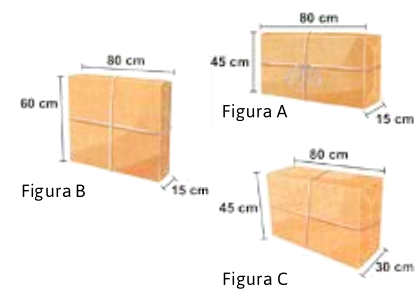
\includegraphics[width=.6\linewidth]{figuras_cajas.png}
                  \captionof{figure}{}
                  \label{fig:figuras_cajas}
              \end{figure}
              \begin{enumerate}
                  \item ¿Qué cantidad de cordón ocupará Pablo?
                  \item El paquete de la figura B es 15 cm más alto que el de la figura A. ¿Cuánto cordón más, del que ocupó en el primero, necesita Pablo para amarrarlo?
                  \item El paquete de la figura C es 15 cm más ancho que el de la figura A. ¿Cuánto cordón más, del que ocupó en el primero, necesita para amarrarlo?
                  \item En parejas justifiquen por qué el empaque de la figura C requiere más cordón que el de la figura B, aun cuando en ambos casos sólo una de las dimensiones se incrementa en 15 cm.
              \end{enumerate}
    \end{enumerate}
\end{boxK}

\subsubsection{Perímetro y expresiones algebraicas}

\begin{enumerate}
    \begin{minipage}[t]{.2\textwidth}
        \begin{figure}[H]
            \centering
            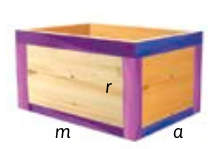
\includegraphics[width=\linewidth]{caja.png}
            \captionof{figure}{}
            \label{fig:caja}
        \end{figure}
    \end{minipage}\hfill
    \begin{minipage}[t]{.7\textwidth}
        \item Sofía compró una caja sin tapa como la de la figura \ref{fig:caja} para guardar fotografías,
        y quiere decorar las orillas de las caras con tiras de tela de colores: de color rosa
        a lo alto, moradas a lo largo y azules a lo ancho.

        \begin{enumerate}
            \item ¿Cuántas tiras de tela ocupará en cada cara de la caja?
            \item ¿Cuántas y de qué color serán las tiras de tela que ocupará?
        \end{enumerate}
    \end{minipage}

    \item Considera que la caja mide $r$ centímetros de alto, $m$ centímetros de largo
          y $a$ centímetros de ancho. Completa la tabla, expresa con esas letras el perímetro
          de una de las caras que se adornarán con las tiras indicadas.
          \begin{figure}[H]
              \centering
              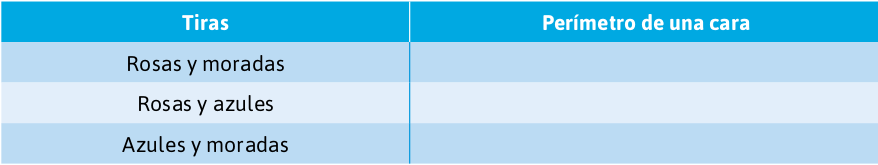
\includegraphics[width=.65\linewidth]{tabla_caja.png}
              \captionof{figure}{}
              \label{fig:tabla_caja}
          \end{figure}
          \begin{enumerate}
              \item Representen con las expresiones anteriores, el perímetro de todas las caras de la
                    caja.
              \item ¿Cuántas tiras de cada color necesita Sofía para adornar toda la caja?
              \item En grupo compartan sus respuestas y validen cada una de ellas. Expresen con
                    las letras $r$, $m$ y $a$ el total de tiras necesarias para adornar la caja.
          \end{enumerate}

          \begin{boxH}
              Una \textbf{expresión algebraica} es una combinación de literales (letras) para representar
              cantidades, y coeficientes (números) junto a ellas que indican cuántas veces se
              multiplica esa cantidad. La letra y el número forman un \textbf{término algebraico}.
          \end{boxH}

          \begin{boxH}
              Los términos algebraicos que tienen las mismas literales se conocen como \textbf{términos semejantes},
              y se simplifican sumando los coeficientes, por ejemplo, \[ 3a + 2a = 5a \].
          \end{boxH}

    \item Pedro, el hermano de Sofía, compró una caja de igual tamaño, y a partir de la idea de
          su hermana, optó por adornar con tiras de color azul, tanto el largo como el ancho de
          la caja y de verde los segmentos verticales.

          \begin{minipage}[t]{0.3\textwidth}
              \begin{figure}[H]
                  \centering
                  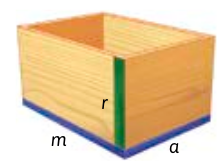
\includegraphics[width=\linewidth]{caja_sintapa.png}
                  \captionof{figure}{}
                  \label{fig:caja_sintapa}
              \end{figure}
          \end{minipage}\hfill
          \begin{minipage}[t]{0.7\textwidth}
              \begin{enumerate}
                  \item Expresa algebraicamente la longitud total de la tira azul que se muestra en la figura \ref{fig:caja_sintapa}.
                  \item Usa tu respuesta anterior para expresar algebraicamente el total de tela azul que
                        Pedro necesitará para decorar su caja.
                  \item Expresa algebraicamente el total de tela (azul y verde) que Pedro utilizará para decorar su caja.
                  \item Compara tu respuesta al inciso anterior con la que diste en el inciso (a de la actividad 2.
                        Escribe tus conclusiones en tu cuaderno.
                  \item Si las cajas miden 12 cm de ancho, 20 cm de largo y 15 cm de alto, ¿cuánta tela ocuparán Sofía y Pedro?
              \end{enumerate}
          \end{minipage}


    \item Julián pintará en la pared una flecha, como la que aparece en la figura \ref{fig:flecha}.
          Para no rebasar los bordes colocará cinta adhesiva alrededor como se observa.

          \begin{minipage}[t]{0.3\textwidth}
              \begin{figure}[H]
                  \centering
                  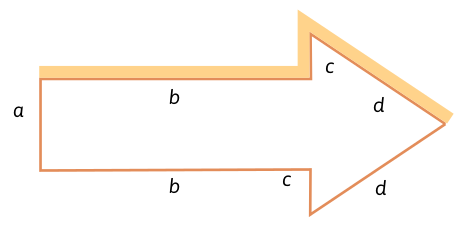
\includegraphics[width=\linewidth]{flecha.png}
                  \captionof{figure}{}
                  \label{fig:flecha}
              \end{figure}
          \end{minipage}\hfill
          \begin{minipage}[t]{0.7\textwidth}
              \begin{enumerate}
                  \item En equipos expresen algebraicamente la cantidad de cinta adhesiva que ya colocó Julián.
                  \item ¿Cuántas veces se debe colocar la cantidad $b + c + d$ de cinta alrededor de la flecha?
                  \item Expresen algebraicamente el total de cinta que Julián colocará alrededor de la flecha.
                  \item ¿Cuál es el perímetro de la figura \ref{fig:flecha}?
              \end{enumerate}
          \end{minipage}

          \begin{boxH}
              Una expresión algebraica cuyos términos tienen el mismo coeficiente es
              equivalente a un producto cuyos factores son el coeficiente y la expresión formada por
              las literales de la expresión original. Por ejemplo,
              \[ 2b + 2c + 2d = 2(b + c + d)\]
          \end{boxH}

          \begin{boxE}
              En las expresiones algebraicas, por simplicidad, para indicar un producto, las literales y los
              coeficientes se escriben juntos; por ejemplo,\\
              \[ 4 \times a = 4a \]
              También se usan paréntesis:\\
              \[ a \times b = (a) (b)\]
          \end{boxE}

    \item Juan y Luis necesitan rodear sus terrenos con una reja de alambre para que pasten
          sus vacas. El terreno de Juan tiene una forma aproximada a la figura \ref{fig:polygon1} y todos sus
          lados miden 22.5 m. El terreno de Luis tiene la forma de la figura \ref{fig:polygon2}, tres de sus
          lados miden 22.5 m y los otros dos, 45 m cada uno.

          \begin{minipage}{0.45\textwidth}
              \begin{figure}[H]
                  \centering
                  
\includegraphics[width=.45\linewidth]{polygon1.png}
                  \captionof{figure}{}
                  \label{fig:polygon1}
              \end{figure}
          \end{minipage}\hfill
          \begin{minipage}{0.45\textwidth}
              \begin{figure}[H]
                  \centering
                  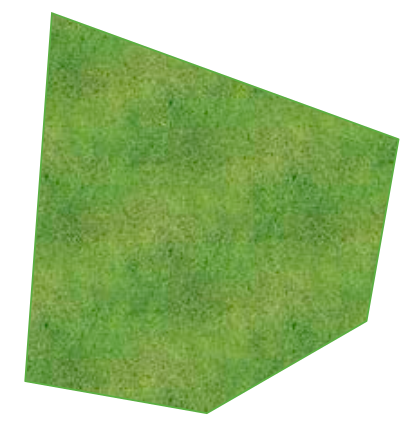
\includegraphics[width=.45\linewidth]{polygon2.png}
                  \captionof{figure}{}
                  \label{fig:polygon2}
              \end{figure}
          \end{minipage}

          \begin{enumerate}
              \item ¿Cuál es la longitud de la reja que Juan necesita para cercar su terreno?
              \item ¿Cuánta reja requiere Luis para cercar el suyo?
              \item Comparte tus procedimientos con un compañero. ¿Los consideran correctos? ¿Por qué?
          \end{enumerate}
    \item En parejas representen algebraicamente la longitud de uno de los lados y el perímetro de todo el terreno de Juan.
          \begin{enumerate}
              \item ¿Cuál de las longitudes del terreno de Luis será más adecuada para representar con la misma literal de tu
                    respuesta anterior? ¿Por qué?
              \item Representen con una literal distinta la longitud mayor del terreno de Luis y expresen algebraicamente su
                    perímetro.
              \item ¿Qué relación hay entre las longitudes de los lados distintos del terreno de Luis?
              \item A partir de su respuesta anterior, reescriban la expresión para el perímetro del terreno de Luis,
                    pero usando una sola literal.
              \item ¿Cómo son entre sí las expresiones de los incisos b) y d)?
              \item ¿Qué cantidad de reja requieren Juan y Luis para rodear sus terrenos? Calculen a partir de las
                    expresiones algebraicas que propusieron.
          \end{enumerate}

          \begin{boxH}
              Si dos variables están relacionadas, una de ellas se puede sustituir por la otra dentro
              de una expresión algebraica. Por ejemplo, si a es igual a $3b$, entonces la expresión
              $a + b$ es equivalente a $3b + b$, porque sustituimos a por $3b$.
              Un término algebraico en el que aparecen dos coeficientes se simplifica multiplicando
              los coeficientes, por ejemplo $3(4a)$ es equivalente a $12a$.
          \end{boxH}

          \subsubsection{El perímetro de un polígono regular}
          Una telaraña se forma por una sucesión de hexágonos regulares tales que la longitud de los
          lados de cada hexágono se incrementa en la misma cantidad con respecto a los lados del
          hexágono anterior (figura \ref{fig:web}).
          \begin{figure}[H]
              \centering
              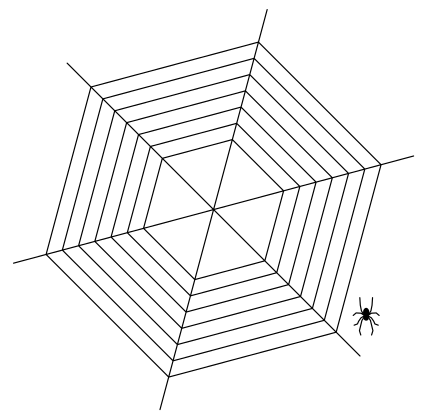
\includegraphics[width=.35\linewidth]{web.png}
              \captionof{figure}{}
              \label{fig:web}
          \end{figure}
          \begin{enumerate}
              \item En parejas escriban una expresión algebraica para representar
                    el perímetro del hexágono más pequeño.
              \item Expresen algebraicamente la longitud de un lado del segundo
                    hexágono a partir de la longitud de un lado del primero.
              \item Completen la tabla \ref{tab:tabla_web}.
                    \begin{figure}[H]
                        \centering
                        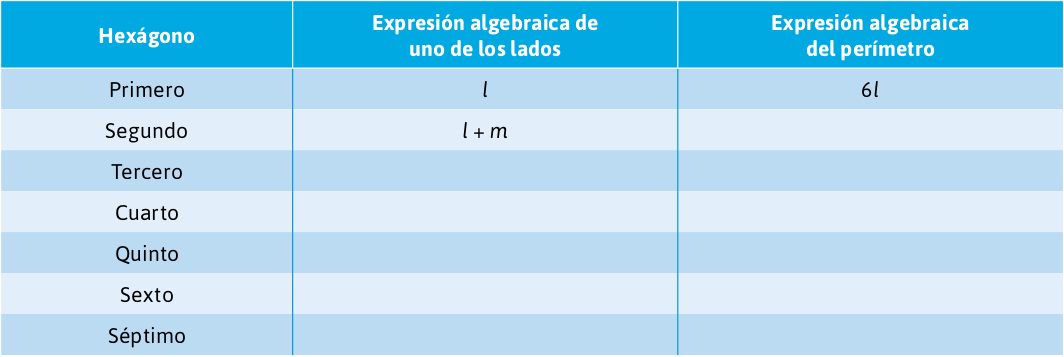
\includegraphics[width=.75\linewidth]{tabla_web.png}
                        \captionof{table}{}
                        \label{tab:tabla_web}
                    \end{figure}
              \item Usa las expresiones anteriores para representar el total de hilo que ha segregado
                    la araña. Simplifica los términos semejantes.
              \item Supón que el lado del hexágono menor mide 4.2 mm y el lado de cada hexágono
                    subsecuente se incrementa en 8 mm, ¿cuáles son los perímetros de los diferentes
                    hexágonos? Anótenlos en la tabla \ref{tab:tabla_lados}.
                    \begin{figure}[H]
                        \centering
                        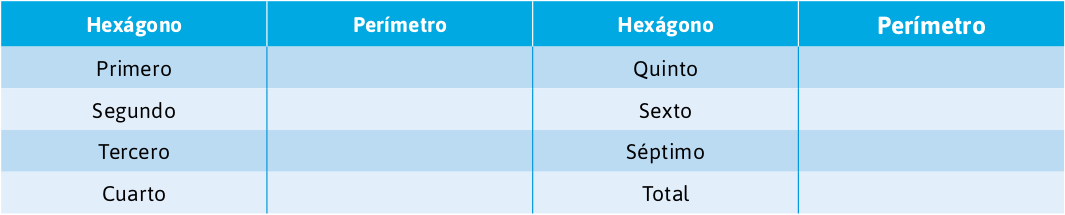
\includegraphics[width=.75\linewidth]{tabla_lados.png}
                        \captionof{table}{}
                        \label{tab:tabla_lados}
                    \end{figure}
              \item Comparen en grupo sus respuestas y procedimientos. ¿Coincidieron los resultados?,
                    ¿por qué? ¿Son iguales las expresiones algebraicas que propusieron? ¿Ocurrió que
                    las expresiones fueran distintas, pero los resultados iguales? Si fue así, justifiquen
                    esa situación; si no, encuentren el error.
              \item ¿Qué cantidad de hilo usó la araña para formar los hexágonos?
          \end{enumerate}
    \item Completa la tabla \ref{tab:tabla_polygons}.
          \begin{figure}[H]
              \centering
              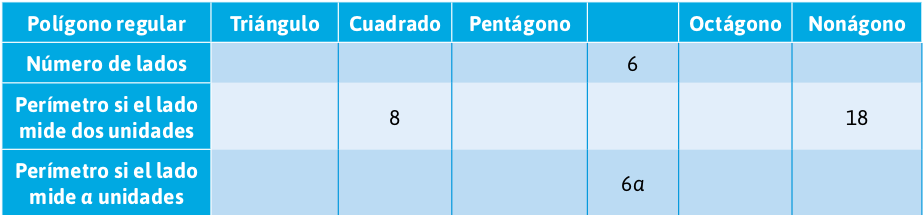
\includegraphics[width=.75\linewidth]{tabla_polygons.png}
              \captionof{table}{}
              \label{tab:tabla_polygons}
          \end{figure}
          \begin{enumerate}
              \item Determina una expresión algebraica para el perímetro de un polígono regular de $n$ lados.
          \end{enumerate}

          \begin{boxH}
              El perímetro de un polígono regular se calcula multiplicando la longitud de un
              lado por el número de lados de los que está compuesto.
          \end{boxH}

    \item Maribel compró una cuerda para forrar las cuatro caras laterales de una caja cúbica de 15 cm de lado.
          Con esa cuerda pudo rodear 30 veces la caja, pero le faltan
          por cubrir 5 cm a lo alto. Observa la figura \ref{fig:boxes}.

          \begin{minipage}{0.25\textwidth}
              \begin{figure}[H]
                  \centering
                  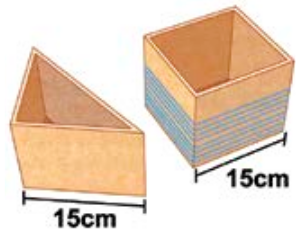
\includegraphics[width=\linewidth]{boxes.png}
                  \captionof{figure}{}
                  \label{fig:boxes}
              \end{figure}
          \end{minipage}\hfill
          \begin{minipage}{0.65\textwidth}
              \begin{enumerate}
                  \item Maribel tiene otra caja con forma de prisma triangular que también mide
                        15 cm de lado. En equipos respondan: ¿en este caso sí le alcanzará la
                        cuerda para cubrir por completo la caja? Expliquen.
                  \item ¿Cuál es el perímetro de la cara inferior de la caja cúbica?
                  \item ¿Cuál es la longitud de la cuerda?
                  \item ¿Cuál es el perímetro de la cara inferior de la caja con forma de prisma triangular?
                  \item ¿Cuál es el perímetro de la cara inferior de la caja con forma de prisma triangular?
                  \item A partir de sus respuestas a los incisos b), c) y d) escriban una justificación o corrijan
                        sus respuestas al inciso a).
              \end{enumerate}
          \end{minipage}

    \item Observa en la figura \ref{fig:hexagon} que los lados del hexágono regular grande miden el triple
          que los lados del hexágono regular pequeño. ¿Cuántas veces es más grande el perímetro del
          hexágono mayor respecto al del hexágono pequeño?

          \begin{minipage}{0.25\textwidth}
              \begin{figure}[H]
                  \centering
                  
\includegraphics[width=\linewidth]{hexagon.png}
                  \captionof{figure}{}
                  \label{fig:hexagon}
              \end{figure}
          \end{minipage}\hfill
          \begin{minipage}{0.65\textwidth}
              \begin{enumerate}
                  \item Escribe una expresión algebraica para el perímetro del hexágono pequeño a partir de la longitud de uno de sus lados.
                  \item Expresa en términos de la longitud de los lados del hexágono pequeño la longitud de un lado del hexágono grande.
                  \item Expresa algebraicamente el perímetro del polígono grande en términos de la longitud del hexágono pequeño.
                  \item Compara tus respuestas y valídenlas con el grupo.
              \end{enumerate}
          \end{minipage}

    \item  Cinco amigos colocan sus toallas de baño sobre la playa formando un gran cuadrado como el de la figura \ref{fig:toallas}.
          Las toallas de Alicia y Beatriz son cuadradas, cada
          una de 720 cm de perímetro, mientras que las de Carlos, Diana y Emilio son rectangulares e iguales.
          \begin{minipage}{0.25\textwidth}
              \begin{figure}[H]
                  \centering
                  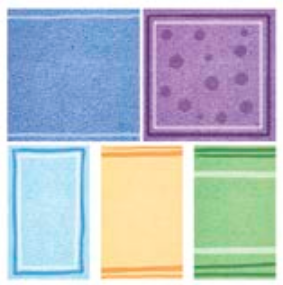
\includegraphics[width=\linewidth]{toallas.png}
                  \captionof{figure}{}
                  \label{fig:toallas}
              \end{figure}
          \end{minipage}\hfill
          \begin{minipage}{0.65\textwidth}
              \begin{enumerate}
                  \item En equipos escriban una expresión algebraica que represente el perímetro de una de las toallas cuadradas si desconocen la longitud de sus lados.
                  \item ¿Cuál es la longitud de los lados de las toallas de Alicia y Beatriz? Expliquen su procedimiento para obtener la respuesta.
                  \item Escriban una expresión con las literales de la expresión algebraica del inciso a que represente el perímetro de las toallas rectangulares.
                  \item Calculen las dimensiones de las toallas rectangulares. Expliquen su procedimiento.
              \end{enumerate}
          \end{minipage}

\end{enumerate}

\begin{boxK}
    \begin{center}\textbf{Cierre}\end{center}

    \begin{enumerate}
        \item Regresa a la sección Inicio y considera que las dimensiones de un paquete son $l$ cm de largo, $a$ cm de ancho y $h$ cm de alto.
              \begin{enumerate}
                  \item Escribe una expresión algebraica que represente el total
                        de cordón necesario para amarrar el empaque.
                  \item Explica el efecto de incrementar cada una de las dimensiones de la caja en la cantidad de cordón necesario
                        para amarrarla.
              \end{enumerate}
        \item En la figura \ref{fig:cuadrados}, I, II, III y IV son cuadrados. Si el perímetro del cuadrado I es 16 cm y
              el del cuadrado II, 24 cm, ¿cuál es el perímetro del cuadrado IV?
              \begin{figure}[H]
                  \centering
                  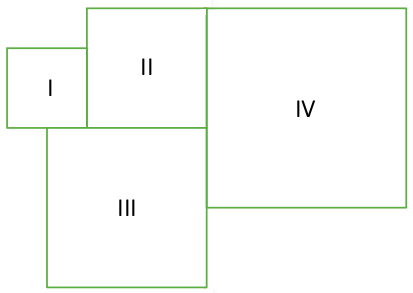
\includegraphics[width=.25\linewidth]{cuadrados.png}
                  \captionof{figure}{}
                  \label{fig:cuadrados}
              \end{figure}
        \item Dado un rectángulo con base $a$ y altura $b$, como el de la figura \ref{fig:rectangulo}
              escribe tres expresiones algebraicas que
              representen el perímetro de la figura \ref{fig:rectangulo}.
              \begin{figure}[H]
                  \centering
                  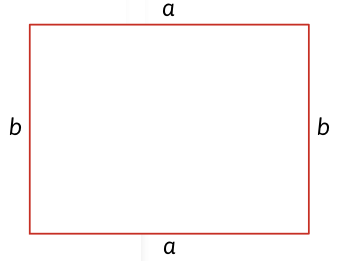
\includegraphics[width=.25\linewidth]{rectangulo.png}
                  \captionof{figure}{}
                  \label{fig:rectangulo}
              \end{figure}
        \item Dos hormigas van del punto A al punto B (figura \ref{fig:hormigas}).
              \begin{figure}[H]
                  \centering
                  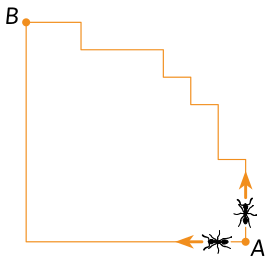
\includegraphics[width=.25\linewidth]{hormigas.png}
                  \captionof{figure}{}
                  \label{fig:hormigas}
              \end{figure}
              \begin{enumerate}
                  \item ¿Qué hormiga recorre un trayecto más largo? Justifica su respuesta.
              \end{enumerate}
    \end{enumerate}
\end{boxK}


\subsection{Perímetro del círculo}

\begin{boxK}
    \begin{center}\textbf{Inicio}\end{center}

    \begin{enumerate}
        \item Ciro tiene un pequeño balón de basquetbol y necesita un aro de alambrón para encestarlo.
              Su balón mide 38 cm de circunferencia y un buen
              reto es encestarlo en un aro cuyo radio sea 5 cm más grande que el del
              balón.
              \begin{figure}[H]
                  \centering
                  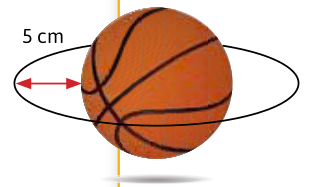
\includegraphics[width=.35\linewidth]{balon.png}
                  \captionof{figure}{}
                  \label{fig:balon}
              \end{figure}
              \begin{enumerate}
                  \item ¿Qué cantidad de alambrón necesitará para elaborar su aro? Explica tu respuesta.
              \end{enumerate}
    \end{enumerate}
\end{boxK}

\begin{enumerate}
    \item Para medir el perímetro de figuras cuyo contorno está formado por segmentos
          rectos se puede usar una regla rígida. Cuando el contorno de una figura es
          curvo necesitamos recurrir a instrumentos flexibles, como las cintas métricas
          de los sastres.
          \begin{enumerate}
              \item En parejas midan el contorno de objetos circulares como los que se mencionan en
                    la primera fila de la tabla. Escriban los datos correspondientes y realicen las
                    operaciones para completar la tabla \ref{tab:tabla_rigidos}.\\

                    \begin{figure}[H]
                        \centering
                        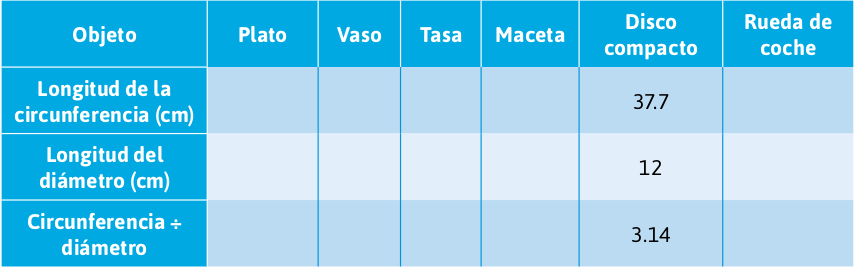
\includegraphics[width=.65\linewidth]{tabla_rigidos.png}
                        \captionof{table}{}
                        \label{tab:tabla_rigidos}
                    \end{figure}

              \item Comparte en grupo los resultados de la última fila. ¿Qu\'e observas? Escribe una conclusión.
              \item En una calculadora científica oprime la tecla del símbolo $\pi$. ¿Qué valor se muestra? Anótenlo.
              \item Compara ese valor con los que obtuviste en la última fila de la tabla. ¿Qué observas?
                    Escriban una conclusión entre todos.
          \end{enumerate}

          \begin{boxH}
              Desde la Antigüedad se sabe que en cualquier círculo hay una relación entre la longitud de la
              circunferencia y la longitud de su diámetro; a saber, la razón entre el perímetro del círculo y
              la longitud de su diámetro es constante.
              Este valor se denota con la letra griega $\pi$ (pi) y es un número decimal infinito no periódico
              cuyas primeras cifras son 3.14159\dots
              Para calcular el perímetro de un círculo, es decir, la longitud de su circunferencia utilizamos
              la expresión $P =\pi d$, donde d es la longitud del diámetro. ¿Por qué esa expresión es correcta?
          \end{boxH}

    \item En la figura \ref{fig:polygons_inside} están inscritos en el círculo un cuadrado,
          un octágono regular y un polígono regular de 16 lados.

          \begin{minipage}{0.3\textwidth}
              \begin{figure}[H]
                  \centering
                  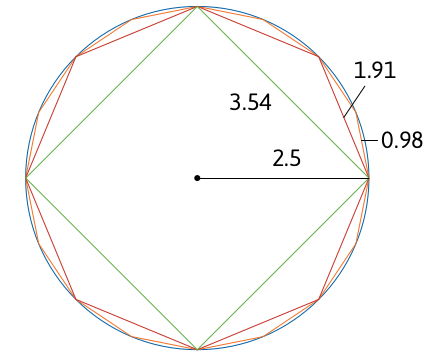
\includegraphics[width=\linewidth]{polygons_inside.png}
                  \captionof{figure}{}
                  \label{fig:polygons_inside}
              \end{figure}
          \end{minipage}\hfill
          \begin{minipage}{0.7\textwidth}
              \begin{enumerate}
                  \item Calcula el perímetro de cada uno.
                  \item Calcula el perímetro del círculo.
                  \item Compara el perímetro de los polígonos con el perímetro del círculo. ¿Qué observas?
                  \item Imagina un polígono regular de 32 lados inscrito en el círculo. ¿Cuál consideras
                        que será el valor aproximado de su perímetro? Justifica tu respuesta y compártela con el grupo.
              \end{enumerate}
          \end{minipage}

          \begin{boxH}
              Medir círculos con precisión es difícil, por eso desde la Antigüedad se propusieron
              métodos para calcular el perímetro de un círculo. Por ejemplo, Arquímedes, usando
              polígonos regulares \textbf{\color{cyan}inscritos y circunscritos} en una circunferencia, obtuvo una muy
              buena aproximación al número $\pi$. Demostró que su valor era un número entre $\frac{223}{71}$ y $\frac{21}{7}$.
              ¿Crees que esa aproximación sea correcta?
          \end{boxH}

          \begin{boxE}
              Polígonos \textbf{\color{cyan}inscritos y cirncunscritos}. Se dice que una figura esta inscrita en otra si cada
              uno de los vértices de la primera figura esta sobre el lado respectivo de la segunda figura.
              En esta misma situación se dice que la segunda figura esta circunscrita en la primera.
          \end{boxE}

          \begin{minipage}[t]{0.7\textwidth}
              \item En una casa de moneda necesitan estuches circulares de
              plástico para guardar centenarios, una moneda de oro mexicana cuya circunferencia es de 11.62 cm (figura \ref{fig:moneda}). ¿Cuál
              es el radio interior mínimo que deben tener un estuche para guardar este tipo de monedas?
          \end{minipage}\hfill
          \begin{minipage}[t]{0.2\textwidth}
              \begin{figure}[H]
                  \centering
                  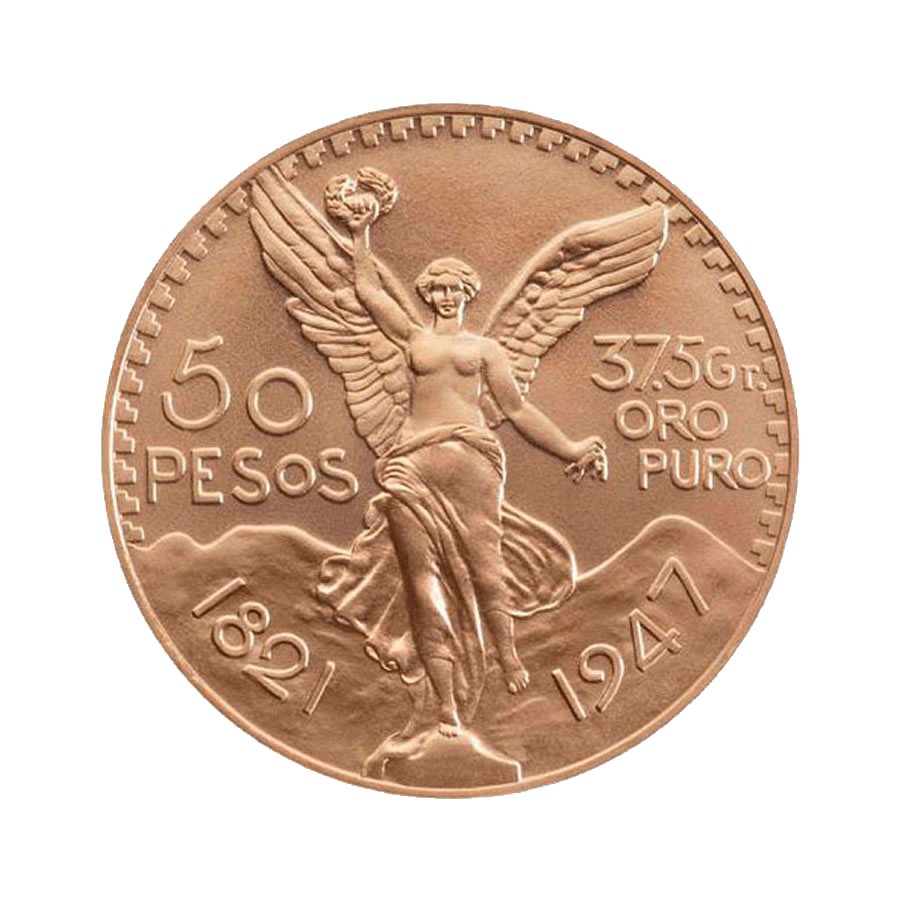
\includegraphics[width=\linewidth]{moneda.png}
                  \captionof{figure}{}
                  \label{fig:moneda}
              \end{figure}
          \end{minipage}



          \begin{minipage}[t]{0.7\textwidth}
              \item Una pista de atletismo debe tener dos partes rectas y dos partes formadas por
              semicírculos. Cada una de las rectas debe medir 100 m de largo, y la longitud de
              cada semicírculo también debe ser de 100 m (figura \ref{fig:pista}). ¿Cuánto mide el radio de los semicírculos?
          \end{minipage}\hfill
          \begin{minipage}[t]{0.2\textwidth}
              \begin{figure}[H]
                  \centering
                  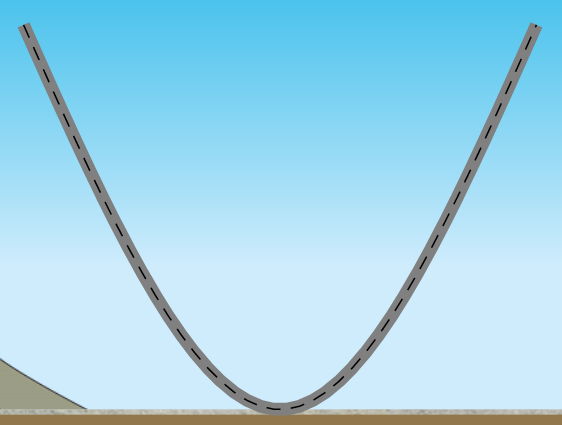
\includegraphics[width=\linewidth]{pista.png}
                  \captionof{figure}{}
                  \label{fig:pista}
              \end{figure}
          \end{minipage}

          \begin{minipage}[t]{0.2\textwidth}
              \begin{figure}[H]
                  \centering
                  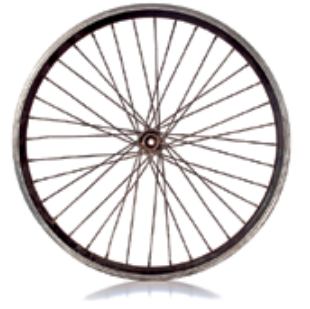
\includegraphics[width=\linewidth]{rueda.png}
                  \captionof{figure}{}
                  \label{fig:rueda}
              \end{figure}
          \end{minipage}\hfill
          \begin{minipage}[t]{0.7\textwidth}
              \item Una rueda de bicicleta está formada por un buje central donde se enganchan los
              rayos. El otro extremo de los rayos se sujetan a un aro metálico donde se coloca
              la llanta (figura \ref{fig:rueda}). Considera que el diámetro de la llanta es de 71.12 cm.

              \begin{enumerate}
                  \item ¿Qué distancia recorre la bicicleta cuando la llanta da una vuelta completa?\\
                  \item ¿Qué distancia recorre si las llantas dan diez vueltas completas?\\
                  \item ¿Cuántas vueltas deben dar las llantas para recorrer un kilómetro?\\
                  \item Los odómetros de los automóviles son instrumentos que miden la distancia que éste
                        recorre y normalmente están conectados a mecanismos de las llantas. Explica su funcionamiento.
              \end{enumerate}
          \end{minipage}

          \begin{minipage}[t]{0.7\textwidth}
              \item Sofía hace un diseño con círculos y semicírculos, como en la figura \ref{fig:jinjang}, y piensa
              cubrir las líneas del círculo y de los semicírculos con cordón dorado.
              \begin{enumerate}
                  \item ¿Cuánto cordón necesitará para cubrir la circunferencia más grande?\\
                  \item ¿Y para cubrir los dos semicírculos interiores?\\
                  \item ¿Qué relación hay entre la longitud del círculo y las de los semicírculos? Explica tu respuesta.
              \end{enumerate}
          \end{minipage}\hfill
          \begin{minipage}[t]{0.2\textwidth}
              \begin{figure}[H]
                  \centering
                  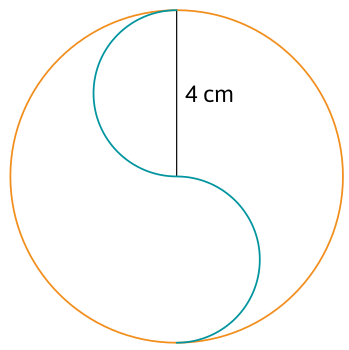
\includegraphics[width=\linewidth]{jinjang.png}
                  \captionof{figure}{}
                  \label{fig:jinjang}
              \end{figure}
          \end{minipage}


    \item Un autódromo tiene la forma y las dimensiones que ilustra la figura \ref{fig:autodromo}.
          \begin{figure}[H]
              \centering
              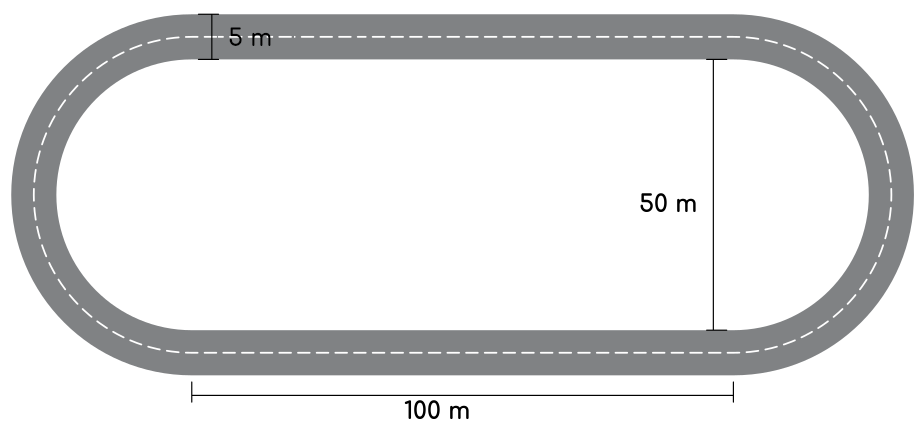
\includegraphics[width=.8\linewidth]{autodromo.png}
              \captionof{figure}{}
              \label{fig:autodromo}
          \end{figure}
          \begin{enumerate}
              \item Calcula la distancia que cubre un auto al recorrer una vez el circuito por el carril interno.\\
              \item Calcula la distancia que se recorre en un auto al conducir una vez por el carril externo.\\
              \item A qué distancia se deben separar dos autos en una carrera de una vuelta para que ambos recorran la misma distancia.
          \end{enumerate}
    \item Carlos mandó construir una ventana con la forma y las medidas que aparecen en
          la figura \ref{fig:ventana}. ¿Qué longitud de material fue necesario para formar el contorno de la ventana?

          \begin{figure}[H]
              \centering
              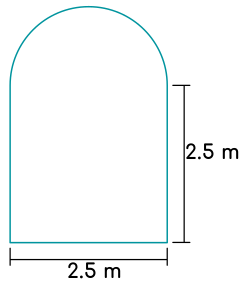
\includegraphics[width=.3\linewidth]{ventana.png}
              \captionof{figure}{}
              \label{fig:ventana}
          \end{figure}
          \newpage
    \item Se construyó una cancha de basquetbol (figura \ref{fig:cancha}) y se quieren pintar todas sus
          líneas: círculo central, área de foul, línea de tres puntos, etcétera. Calcula la longitud de todas las líneas que se deben pintar.
          \begin{figure}[H]
              \centering
              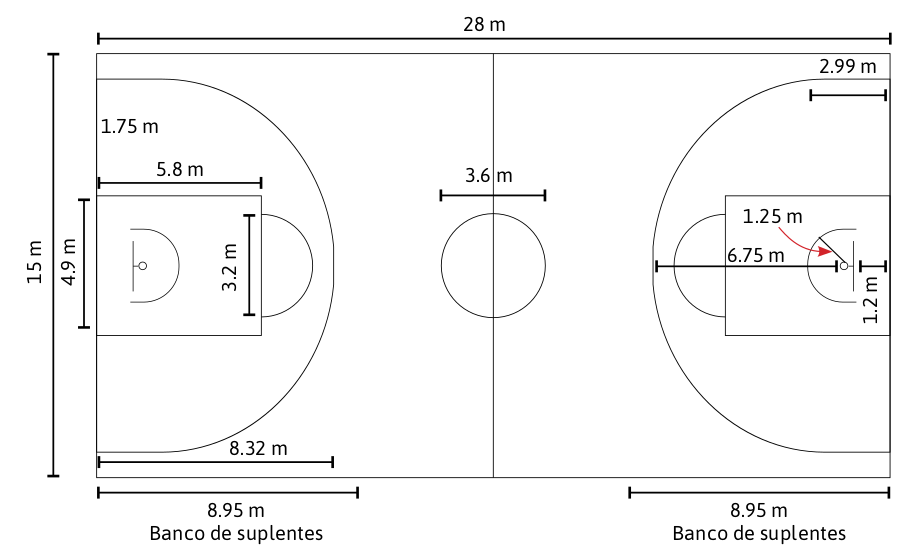
\includegraphics[width=.8\linewidth]{cancha.png}
              \captionof{figure}{}
              \label{fig:cancha}
          \end{figure}

    \item En equipos compartan y validen sus respuestas a los ejercicios del 3 al 9. Organícense
          para que cada equipo exponga la solución de un ejercicio al resto del grupo.
\end{enumerate}

\begin{boxK}
    \begin{center}\textbf{Cierre}\end{center}
    \begin{enumerate}
        \item Regresa a la situación de Inicio y determina el diámetro del balón de Ciro.
              \begin{enumerate}
                  \item ¿Cuánto debe medir el diámetro del aro?
                  \item ¿Qué tanto alambrón necesita Ciro para el aro?
              \end{enumerate}
        \item Un avión supersónico dará una vuelta alrededor de la Tierra sobre el
              ecuador a una altura promedio de 10,000 m. Considera que la circunferencia de la Tierra es de 40,066.4 km.
              \begin{enumerate}
                  \item ¿Qué distancia habrá recorrido el avión al cumplir su objetivo?
              \end{enumerate}
        \item Las ciudades de Chicago y Estambul están sobre un mismo paralelo de
              nuestro planeta. Si el radio de la circunferencia que constituye ese
              paralelo es de 4,000 km:
              \begin{enumerate}
                  \item ¿Qué distancia se debe recorrer sobre la superficie de la Tierra para
                        ir de una ciudad a otra sobre ese paralelo? Considera que los radios
                        del centro de la Tierra hacia las ciudades forman un ángulo de 120°,
                        esto es, la distancia entre ellas es la tercera parte del paralelo.
              \end{enumerate}
        \item Comparte y valida tus respuestas con el resto de tus compañeros.
    \end{enumerate}
\end{boxK}

\newpage
\subsection{Áreas de triángulos y cuadriláteros}

\begin{boxK}
    \begin{center}\textbf{Inicio}\end{center}

    \begin{enumerate}
        \item Un arquitecto diseña dos escuelas que se construirán en terrenos como las figuras \ref{fig:arqui}.
              \begin{figure}[H]
                  \centering
                  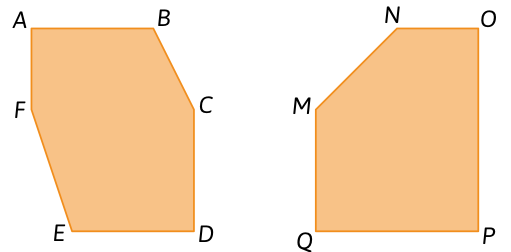
\includegraphics[width=.5\linewidth]{arqui.png}
                  \captionof{figure}{}
                  \label{fig:arqui}
              \end{figure}
              \begin{enumerate}
                  \item Observa ambas figuras. ¿Qué terreno consideras que tiene mayor área? ¿Por qué?
                  \item Realiza las mediciones necesarias y verifica tu respuesta.
                  \item ¿Cómo calculaste el área de las figuras? Explica tu respuesta.
              \end{enumerate}
    \end{enumerate}
\end{boxK}















\newpage

\mychapter{}

\thispagestyle{plain}
\section{Variaciones diversas}

\boxabstract{Aprendizajes esperados:}{Analiza y compara diversos tipos de variación a partir de sus representaciones tabular, gráfica y algebraica, que resultan de modelar situaciones y fenómenos de la Física y de otros contextos.}

\subsection{Interpretación de gr\'aficas}

\begin{boxK}
    \begin{center}\textbf{Inicio}\end{center}

\end{boxK}

\begin{boxK}
    \begin{center}\textbf{Cierre}\end{center}

\end{boxK}

\subsection{Construcción de gr\'aficas a partir de tablas}

\begin{boxK}
    \begin{center}\textbf{Inicio}\end{center}

\end{boxK}

\begin{boxK}
    \begin{center}\textbf{Cierre}\end{center}

\end{boxK}

\subsection{Análisis de gr\'aficas de variaciones diversas}

\begin{boxK}
    \begin{center}\textbf{Inicio}\end{center}

\end{boxK}

\begin{boxK}
    \begin{center}\textbf{Cierre}\end{center}

\end{boxK}

\newpage

\newpage \thispagestyle{plain}
\section{Energía y reacción química}
\subsection{¿Cómo se transfiere energía durante las reacciones químicas?}
\subsection{¿Por qué se transfiere energía durante las reacciones químicas?}

\newpage \thispagestyle{plain}
\section{La energía química en nuestras vidas}
\subsection{¿Cuáles son los beneficios, costos y riesgos de usar energía química?}


\thispagestyle{plain}
\section{Expresiones algebraicas de ecuaciones y funciones}
\subsection{Expresiones algebraicas de ecuaciones}
\subsection{Expresiones algebraicas de funciones}

\newpage

\thispagestyle{plain}
\section{Teorema de Pitágoras}
\subsection{Triángulos rectángulos y el teorema de Pitágoras}
\subsection{El teorema de Pitágoras}
\subsection{Aplicaciones del teorema de Pitágoras}

\newpage

\thispagestyle{plain}
\section{Razones trigonométricas (seno, coseno y tangente)}
\subsection{Razones trigonométricas básicas}
\subsection{Razones trigonométricas de 30$^{\circ}$, 45$^{\circ}$ y 60$^{\circ}$}

\newpage

\thispagestyle{plain}
\section{Resolución de triángulos rectángulos}
\subsection{Seno, coseno y tangente de ángulos agudos}
\subsection{Aplicaciones de razones trigonométricas}
\end{document}